% !TeX root = ../main.tex

\section{Progettazione Logica}

\subsection{Ristrutturazione del modello Entità-Relazione}
A partire dallo schema iniziale è stata effettuata una ristrutturazione del modello con l'obiettivo di ridurre la frammentazione del diagramma e rendere più agevole la successiva traduzione verso il modello logico-relazionale.

La revisione ha riguardato soprattutto i punti in cui il modello originale utilizzava più livelli di specializzazione per rappresentare differenze operative che potevano essere espresse in modo più compatto.

In particolare:
\begin{itemize}
  \item le specializzazioni \textbf{Cassa} e \textbf{Sportello} sono state accorpate nell'unica entità \textbf{Interfaccia}, introducendo l'attributo \textit{Tipo} come discriminante;
  \item la gerarchia di \textbf{Operazioni}, articolata nei sottotipi \textbf{Prelievo}, \textbf{Deposito} e \textbf{Operazioni Sportello}, è stata semplificata in una singola entità \textbf{Operazioni} con attributo \textit{Tipo};
  \item i sottotipi \textbf{Saldo} e \textbf{Lista Movimenti}, originariamente modellati come specializzazioni di \textbf{Operazioni Sportello}, sono stati ricondotti a valori del medesimo attributo \textit{Tipo};
  \item la rappresentazione dei soggetti del sistema è stata resa più lineare attorno all'entità \textbf{Persona}, mantenendo i ruoli di \textbf{Cliente} e \textbf{Impiegato} ma riducendo la complessità grafica complessiva;
\end{itemize}

La ristrutturazione non altera il significato informativo dello schema, ma ne migliora la leggibilità e ne riduce il numero di costrutti specializzati. In questo modo il modello finale risulta più compatto e più facilmente traducibile nello schema logico-relazionale, pur rimanendo coerente con i requisiti della traccia.

\begin{figure}[H]
  \begin{center}
    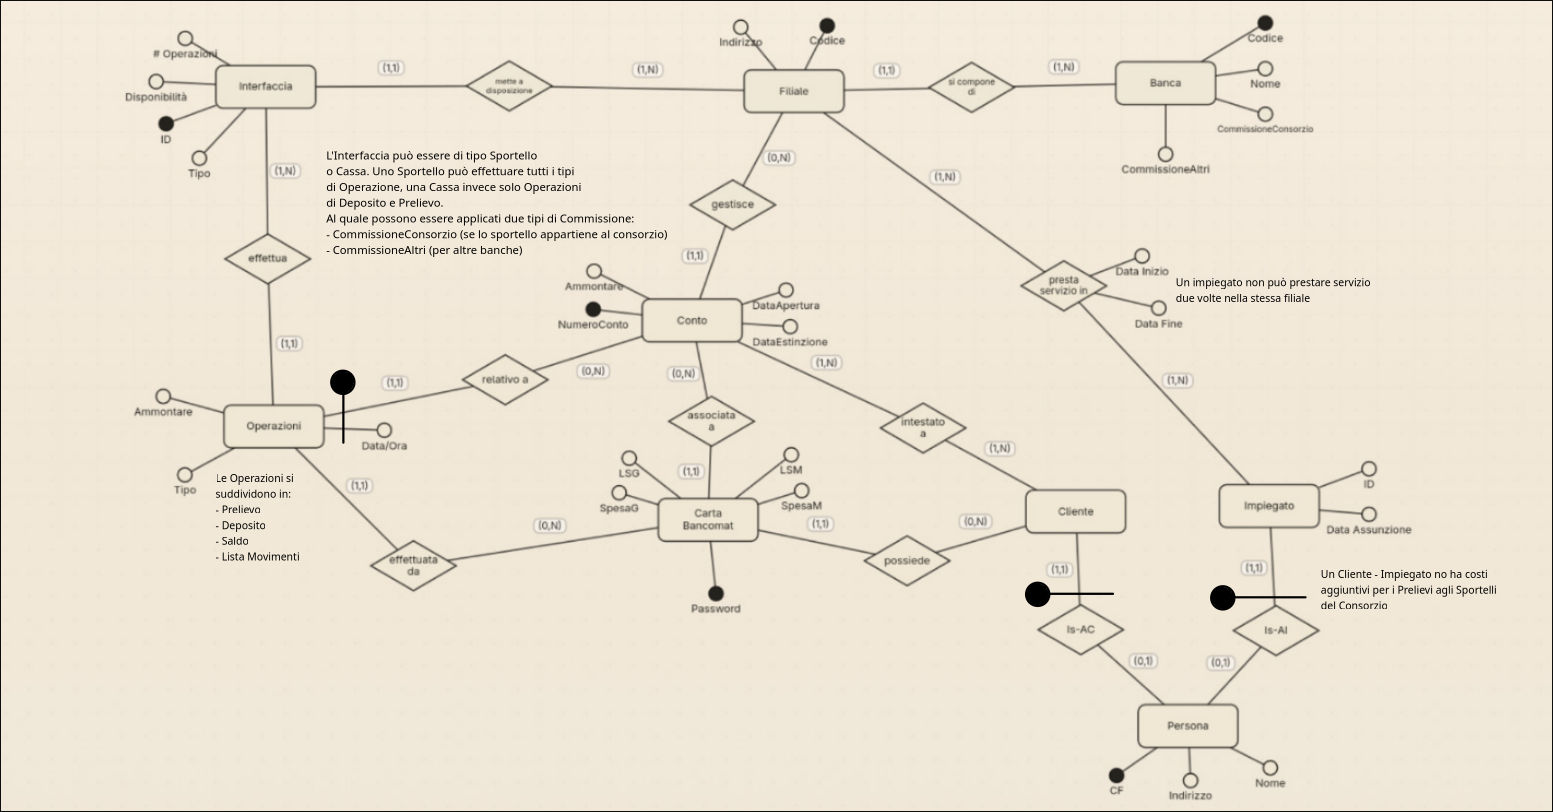
\includegraphics[width=0.95\textwidth]{../imgs/refactorER.png}
  \end{center}
  \caption{Ristrutturazione dello schema Entità-Relazione del Consorzio Bancario}
  \label{fig:ref_er}
\end{figure}


In seguito alla ristrutturazione si procede alla sua traduzione nel modello \textbf{relazionale}. In questa fase, le entità del dominio, le associazioni e i vincoli principali vengono rappresentati mediante relazioni, chiavi primarie, chiavi esterne e, vincoli di integrità.

La traduzione è stata effettuata seguendo i criteri classici:
\begin{itemize}
  \item ogni entità forte è stata trasformata in una relazione;
  \item le relazioni \textit{uno a molti} sono state tradotte riportando la chiave primaria dell'entità dal lato \(1\) come chiave esterna dell'entità dal lato \(N\);
  \item le relazioni \textit{molti a molti} sono state tradotte mediante relazioni autonome;
  \item la generalizzazione \textbf{Persona} -- \textbf{Cliente}/\textbf{Impiegato} è stata realizzata mantenendo una relazione per la superclasse e una per ciascun sottotipo;
  \item le specializzazioni introdotte nel modello concettuale per \textbf{Interfaccia} e \textbf{Operazione} sono state assorbite dall'attributo \textbf{tipo};
\end{itemize}


\subsection{Schema relazionale}

Lo schema logico risultante è il seguente:

\begin{itemize}
  \item \textbf{Banca}(\underline{codiceBanca}, nomeBanca, commissioneAltri, commissioneConsorzio)

  \item \textbf{Filiale}(\underline{codiceFiliale}, indirizzo, \textit{bancaReferente})

  \item \textbf{Persona}(\underline{codiceFiscale}, nome, indirizzo)

  \item \textbf{Cliente}(\underline{\textit{codiceFiscale\_c}})

  \item \textbf{Impiegato}(\underline{\textit{codiceFiscale\_i}}, idImpiegato, dataAssunzione)

  \item \textbf{Conto}(\underline{numeroConto}, dataApertura, dataEstinzione, ammontare, \textit{filialeReferente})

  \item \textbf{Intestato\_A}(\underline{\textit{codiceFiscale\_int}}, \underline{\textit{numeroConto\_int}})

  \item \textbf{CartaBancomat}(\underline{passwordBancomat}, limiteSpesaGiornaliero, limiteSpesaMensile, spesaGiornaliera, spesaMensile, \textit{numeroConto\_cb}, \textit{codiceFiscale\_cb})

  \item \textbf{Interfaccia}(\underline{idInterfaccia}, tipo, disponibilita, numeroOperazioni, \textit{codiceFiliale\_i})

  \item \textbf{Operazione}(\underline{idOperazione}, dataOperazione, oraOperazione, tipo, ammontare, \textit{numeroConto\_o}, \textit{idInterfaccia\_o}, \textit{passwordBancomat})

  \item \textbf{PrestaServizioIn}(\underline{\textit{idImpiegato\_psi}}, \underline{\textit{codiceFiliale\_psi}}, dataInizio, dataFine)
\end{itemize}

Nel precedente schema, gli attributi sottolineati rappresentano le \textbf{chiavi primarie}, mentre quelli in corsivo rappresentano le \textbf{chiavi esterne}.

\subsection{Chiavi esterne e significato delle relazioni}

Le dipendenze referenziali introdotte sono le seguenti:

\begin{itemize}
  \item \textit{bancaReferente} in \textbf{Filiale} referenzia \textbf{Banca}(codiceBanca);
  \item \textit{codiceFiscale\_c} in \textbf{Cliente} referenzia \textbf{Persona}(codiceFiscale);
  \item \textit{codiceFiscale\_i} in \textbf{Impiegato} referenzia \textbf{Persona}(codiceFiscale);
  \item \textit{filialeReferente} in \textbf{Conto} referenzia \textbf{Filiale}(codiceFiliale);
  \item \textit{codiceFiscale\_int} in \textbf{Intestato\_A} referenzia \textbf{Cliente}(codiceFiscale\_c);
  \item \textit{numeroConto\_int} in \textbf{Intestato\_A} referenzia \textbf{Conto}(numeroConto);
  \item \textit{numeroConto\_cb} in \textbf{CartaBancomat} referenzia \textbf{Conto}(numeroConto);
  \item \textit{codiceFiscale\_cb} in \textbf{CartaBancomat} referenzia \textbf{Cliente}(codiceFiscale\_c);
  \item \textit{codiceFiliale\_i} in \textbf{Interfaccia} referenzia \textbf{Filiale}(codiceFiliale);
  \item \textit{numeroConto\_o} in \textbf{Operazione} referenzia \textbf{Conto}(numeroConto);
  \item \textit{idInterfaccia\_o} in \textbf{Operazione} referenzia \textbf{Interfaccia}(idInterfaccia);
  \item \textit{passwordBancomat\_o} in \textbf{Operazione} referenzia \textbf{CartaBancomat}(passwordBancomat);
  \item \textit{idImpiegato\_psi} in \textbf{PrestaServizioIn} referenzia \textbf{Impiegato}(idImpiegato);
  \item \textit{codiceFiliale\_psi} in \textbf{PrestaServizioIn} referenzia \textbf{Filiale}(codiceFiliale).
\end{itemize}

\subsection{Osservazioni sulle scelte di traduzione}

La generalizzazione tra \textbf{Persona}, \textbf{Cliente} e \textbf{Impiegato} è stata mantenuta in modo esplicito, così da poter rappresentare correttamente il caso in cui uno stesso soggetto sia contemporaneamente cliente e impiegato. In questo modo le informazioni anagrafiche comuni sono memorizzate una sola volta nella relazione \textbf{Persona}, evitando ridondanze.

Per l'entità \textbf{Impiegato} è stato introdotto, oltre al codice fiscale ereditato da \textbf{Persona}, anche l'attributo \textit{idImpiegato}, utilizzato come identificatore operativo nelle relazioni di servizio presso le filiali. Tale attributo costituisce una chiave alternativa con vincolo di univocità.

La relazione \textbf{Intestato\_A} realizza l'associazione molti-a-molti tra clienti e conti correnti, in quanto un conto può essere cointestato a più clienti e un cliente può possedere più conti.

L'entità \textbf{CartaBancomat} è stata tradotta in una relazione autonoma collegata sia al conto sia al cliente possessore. Sono stati inoltre mantenuti gli attributi \textit{spesaGiornaliera} e \textit{spesaMensile}, utili al controllo dei limiti operativi della carta.

Le entità \textbf{Cassa} e \textbf{Sportello} del modello concettuale sono state ricondotte alla sola relazione \textbf{Interfaccia}, distinguendo i due casi attraverso l'attributo \textit{tipo}. In modo analogo, i diversi tipi di operazione bancaria sono stati accorpati nella relazione \textbf{Operazione}, ancora una volta tramite l'attributo \textit{tipo}.

L'attributo \textit{ammontare} di \textbf{Operazione} può risultare nullo per operazioni informative come saldo e lista movimenti, mentre assume un valore numerico per depositi e prelievi.

L'attributo \textit{numeroOperazioni} di \textbf{Interfaccia}, pur essendo concettualmente derivabile dal conteggio delle operazioni eseguite, è stato mantenuto nello schema logico in forma memorizzata per motivi di efficienza, delegandone l'aggiornamento automatico alla logica implementativa.

\subsection{Vincoli di integrità non esprimibili direttamente nello schema relazionale}

Alcuni vincoli applicativi non sono esprimibili in modo completo mediante sole chiavi e vincoli referenziali, e richiedono quindi controlli aggiuntivi a livello implementativo:

\begin{itemize}
  \item un impiegato può prestare servizio soltanto presso filiali appartenenti alla banca di riferimento;
  \item un impiegato deve permanere per almeno un mese in una filiale prima di potere essere trasferito;
  \item un impiegato non può essere assegnato nuovamente a una filiale presso cui ha già prestato servizio;
  \item un conto estinto non può essere utilizzato per nuove operazioni;
  \item in caso di estinzione del conto, l'ammontare residuo deve essere nullo oppure pari a zero;
  \item un prelievo non può superare il saldo disponibile del conto;
  \item un prelievo non può superare la disponibilità dell'interfaccia presso cui viene effettuato;
  \item la carta Bancomat utilizzata in un'operazione deve essere associata al conto su cui l'operazione viene eseguita;
  \item l'importo di un prelievo non può eccedere il limite giornaliero o mensile disponibile della carta;
  \item le commissioni sui prelievi dipendono dalla banca proprietaria del conto e dalla banca a cui appartiene l'interfaccia utilizzata;
  \item nel caso in cui un cliente sia anche impiegato della stessa banca, non vengono applicate commissioni per le operazioni effettuate presso filiali della banca stessa o presso sportelli del consorzio.
\end{itemize}

\subsection{Qualità dello schema}
Lo schema risulta regolare e adeguato alla traduzione fisica. La separazione tra \textbf{Persona}, \textbf{Cliente} e \textbf{Impiegato}, così come l'uso di relazioni associative per i legami molti-a-molti, mantiene una struttura coerente con i requisiti della traccia. Alcuni attributi ridondanti sono stati mantenuti consapevolmente per supportare in modo più efficiente controlli e aggiornamenti operativi.
